\documentclass[a4paper, 11pt]{report}


% Language
%->8-------------------------------------------------------------------------------------------8<-%
\usepackage[brazil]{babel}
\usepackage[utf8]{inputenc}
\usepackage[T1]{fontenc}
%->8-------------------------------------------------------------------------------------------8<-%


% Document Structure
%->8-------------------------------------------------------------------------------------------8<-%
\usepackage[a4paper, margin=1in]{geometry}
\usepackage{indentfirst}
\usepackage{changepage}
\setlength{\parskip}{\baselineskip}                              % Space between paragraphs
\newcommand{\nonport}[1]{\textit{#1}}                            % For texts in a foreign language
\renewcommand{\labelenumi}{(\theenumi)}                          % Makes itemize be (number)
\addtolength{\jot}{0.4em}
%->8-------------------------------------------------------------------------------------------8<-%


% TOC Spacing
%->8-------------------------------------------------------------------------------------------8<-%
\usepackage{tocloft, hyperref, tocbibind}
\setlength{\cftbeforechapskip}{12pt}  % Space before chapter's title
\setlength{\cftbeforesecskip}{6pt}    % Space before sections's title
\setlength{\cftbeforesubsecskip}{6pt} % Space before subsections's title
\setlength{\cftchapnumwidth}{3em}     % Space between chapter's number and chapter's title
\setlength{\cftsecnumwidth}{3.5em}    % Space between section's number and section's title
\setlength{\cftsubsecnumwidth}{4em}   % Space between subsection's number and subsection's title
\setlength{\cftchapindent}{0em}       % Space before chapters in TOC
\setlength{\cftsecindent}{3em}        % Space before sections in TOC
\setlength{\cftsubsecindent}{6.5em}   % Space before subsections in TOC
%->8-------------------------------------------------------------------------------------------8<-%


% Bibliography and Figures
%->8-------------------------------------------------------------------------------------------8<-%
\usepackage[backend=biber]{biblatex}
\usepackage{csquotes}
\usepackage{graphicx, float}
\addbibresource{repertoire.bib}
\graphicspath{{figures}}
%->8-------------------------------------------------------------------------------------------8<-%


% Math
%->8-------------------------------------------------------------------------------------------8<-%
\usepackage{amsmath, amssymb, calculation, mathdots, scalerel, mathtools, amsthm}
\newenvironment{jmatrix}{\left[\begin{matrix}}{\end{matrix}\right]}
\newcommand{\norm}[1]{\left\lVert#1\right\rVert}
\newcommand{\fnorm}[1]{\left\lVert#1\right\rVert_\mathsf{F}}
\newcommand{\dist}[1]{\text{dist}(#1)}
\renewcommand{\t}{^{\scriptscriptstyle\mathsf{T}\mkern-1mu}}
\renewcommand{\dim}[2]{(#1 \times #2)}
\renewcommand{\vert}{\rule[-1ex]{0.5pt}{2.5ex}}
\newcommand{\hori}{\rule[.5ex]{2.5ex}{0.5pt}}
\newcommand{\argmin}[1]{\underset{#1}{\text{Argmin}}\,\,}
\newcommand{\grad}[1]{\underset{#1}{\nabla}\,\,}
\newcommand{\var}{\text{Var}}
\newcommand{\expval}{\text{E}}
\newcommand{\st}{\,\,|\,\,}
\newcommand{\impliesdown}{\displaystyle\Downarrow}
\renewcommand{\bar}[1]{\overline{#1}}
%->8-------------------------------------------------------------------------------------------8<-%


% Code
%->8-------------------------------------------------------------------------------------------8<-%
\usepackage{listings}
\lstnewenvironment{code}[1][]{
  \lstset{
    basicstyle=\ttfamily,
    columns=flexible,
    breaklines=true,
    breakatwhitespace=true,
    frame=none,
    basewidth=0.5em,
    aboveskip=13pt,
    belowskip=0pt,
    #1
  }
}{}
%->8-------------------------------------------------------------------------------------------8<-%


\begin{document}

  %->8-------------------------------------------------8<-%
  \title{
    \begin{figure}
      \centering
    \end{figure}
    \Huge{Randomized Matrix Multiplication} \\
    \Huge{Aproximando o Produto Matricial Utilizando Probabilidade}
  }
  \date{\Large{\today \vfill Rio de Janeiro - RJ}}
  \author{
    \LARGE{João Victor Lopez Pereira}
    \vspace{1cm} \\
    \Large{Instituto de Computação} \\
    \Large{Centro de Ciências da Matemática e da Natureza} \\
    \Large{Universidade Federal do Rio de Janeiro}
  }
  \maketitle
  \newpage
  \tableofcontents
  \newpage
  %->8-------------------------------------------------8<-%

  \chapter{Motivação}
    
Dadas duas matrizes $A$ e $B$, ambas de dimensão $\dim{n}{n}$, o algoritmo (tradicional) que computa o produto $AB$ é:

\begin{code}
function matrix_product(A, B)
    n = size(A, 1)
    C = zeros(n, n)
    for i in 1:n
        for j in 1:n
            for k in 1:n
                C[i, j] += A[i, k] * B[k, j]
            end
        end
    end
    return C
end
\end{code}

que, apesar de ser um algoritmo exato, perfeitamente preciso e que segue diretamente da definição matemática de produto matricial, apresenta $3$ \nonport{loops} aninhados, ambos de $1$ a $n$, o que resulta em uma complexidade computacional $O(n^3)$.

De maneira mais precisa, o produto de duas matrizes $A$ e $B$ é dado por

\[
  A B =
  \begin{jmatrix}
  \vert & & \vert \\ a_1 & \dots & a_n \\ \vert & & \vert
  \end{jmatrix}
  \begin{jmatrix}
  \hori & b_1\t & \hori \\
  & \vdots & \\
  \hori & b_n\t & \hori \\
  \end{jmatrix}
  =
  \sum_{i=1}^{n}
  a_i b_i\t.
\]

% mention algoritms with complexity O(n^{2.7})

O produto matricial $AB$ pode ser expresso como sendo a soma de várias matrizes de posto $1$ no formato $a_i b_i\t$, sendo $a_i$ a $i$ésima coluna da matriz $A$ e $b_i$ a $i$ésima linha da matriz $B$. Perceba que diferentes matrizes $a_i b_i\t$ apresentam diferentes contribuições para a formação do produto $AB$ final. Por exemplo:

\begin{calculation}[=]
  \begin{jmatrix}
    10 & 1 \\ 20 & 3
  \end{jmatrix}
  \begin{jmatrix}
    2 & 30 \\ 2 & 0.5
  \end{jmatrix}
  \step{$AB = \displaystyle \sum_{i=1}^{n} a_i b_i\t$}
  \begin{jmatrix}
    10 \\ 20
  \end{jmatrix}
  \begin{jmatrix}
    2 & 30
  \end{jmatrix}
  +
  \begin{jmatrix}
    1 \\ 3
  \end{jmatrix}
  \begin{jmatrix}
    2 & 0.5
  \end{jmatrix}
  \step{Produto}
  \begin{jmatrix}
    20 & 300 \\ 40 & 600
  \end{jmatrix}
  +
  \begin{jmatrix}
    2 & 0.5 \\ 6 & 1.5
  \end{jmatrix}
  \step{Soma índice a índice}
  \begin{jmatrix}
    22 & 300.5 \\ 46 & 601.5
  \end{jmatrix}.
\end{calculation}

Perceba que o produto $a_1b_1\t$ resultou em uma matriz muito mais próxima de $AB$ do que o produto $a_2b_2\t$, e que, consequentemente, sua importância no cálculo de $AB$ foi maior. Podemos, de maneira informal, dizer que

\[
  \begin{jmatrix}
    \vert & \vert \\ a_1 & a_2 \\ \vert & \vert
  \end{jmatrix}
  \begin{jmatrix}
    \hori & b_1\t & \hori \\ \hori & b_2\t & \hori
  \end{jmatrix}
  \approx
  \begin{jmatrix}
    \vert \\ a_1 \\ \vert
  \end{jmatrix}
  \begin{jmatrix}
    \hori & b_1\t & \hori
  \end{jmatrix}
\]
\[
  \begin{jmatrix}
    \vert & \vert \\ a_1 & a_2 \\ \vert & \vert
  \end{jmatrix}
  \begin{jmatrix}
    \hori & b_1\t & \hori \\ \hori & b_2\t & \hori
  \end{jmatrix}
  \approx
  \begin{jmatrix}
    \vert \\ a_2 \\ \vert
  \end{jmatrix}
  \begin{jmatrix}
    \hori & b_2\t & \hori
  \end{jmatrix}.
\]

No caso do exemplo acima, temos

\[
  \begin{jmatrix}
    22 & 300.5 \\ 46 & 601.5
  \end{jmatrix}
  \approx
  \begin{jmatrix}
    10 \\ 20
  \end{jmatrix}
  \begin{jmatrix}
    2 & 30
  \end{jmatrix}
  =
  \begin{jmatrix}
    20 & 300 \\ 40 & 600
  \end{jmatrix}
\]
\[
  \begin{jmatrix}
    22 & 300.5 \\ 46 & 601.5
  \end{jmatrix}
  \approx
  \begin{jmatrix}
    1 \\ 3
  \end{jmatrix}
  \begin{jmatrix}
    2 & 0.5
  \end{jmatrix}
  =
  \begin{jmatrix}
    2 & 0.5 \\ 6 & 1.5
  \end{jmatrix}.
\]

Ou seja,

\[
  \begin{jmatrix}
    22 & 300.5 \\ 46 & 601.5
  \end{jmatrix}
  \approx
  \begin{jmatrix}
    20 & 300 \\ 40 & 600
  \end{jmatrix}
\]
\[
  \begin{jmatrix}
    22 & 300.5 \\ 46 & 601.5
  \end{jmatrix}
  \approx
  \begin{jmatrix}
    2 & 0.5 \\ 6 & 1.5
  \end{jmatrix}.
\]

É visível que, se considerarmos o erro como sendo a norma de Frobenius da diferença entre $AB$ e sua aproximação, ou algum critério de semelhança como sendo a razão entre as normas de Frobenius de $AB$ e sua aproximação, respectivamente, teremos que a matriz resultante de $a_1b_1\t$ apresenta uma aproximação muito melhor para $AB$ do que $a_2b_2\t$.

\[\fnorm{\begin{jmatrix}
    22 & 300.5 \\ 46 & 601.5
  \end{jmatrix}}
  \approx
  674.3
\]
\[\fnorm{\begin{jmatrix}
    20 & 300 \\ 40 & 600
  \end{jmatrix}}
  \approx 672.3
\]
\[
\fnorm{\begin{jmatrix}
    2 & 0.5 \\ 6 & 1.5
  \end{jmatrix}}
  \approx 6.5.
\]

Podemos atribuir essa melhor representação devido à magnitude dos elementos de $a_1 b_1\t$, que se assemelham aos elementos de $AB$.

Nesse exemplo, em específico, a dimensão das matrizes $A$ e $B$ foram pequenas, de modo que o custo $O(n^3)$ seja quase desconsiderável. Ainda assim, em um produto entre matrizes com dimensões muito maiores em que diferentes matrizes de posto $1$ no formato $a_ib_i\t$ apresentem importância significativa em comparação com as demais, é razoável que o produto $AB$ seja aproximado por meio de $s$ amostras de matrizes $a_ib_i\t$ amostradas, resultando em uma aproximação \[\sum_{k=1}^{s} a_{i_{k}} b_{i_{k}}\t,\] sendo $i_k$ o resultando da $k$ésima amostra, resultando assim em uma complexidade computacional $O(sn^2)$, com $s$ necessariamente menor do que $n$ (caso contrário, o produto matricial tradicional faria muito mais sentido).

Em outras palavras, temos que o produto das matrizes de dimensão $\dim{n}{n}$ é expresso como a soma de $n$ matrizes, das quais gostaríamos de escolher probabilisticamente as mais importantes para aproximar o produto $AB$ final.

No exemplo anterior, por exemplo, temos que

\[
  \underbrace{\begin{jmatrix}
    22 & 300.5 \\ 46 & 601.5
  \end{jmatrix}}_{AB}
  =
  \underbrace{\begin{jmatrix}
    20 & 300 \\ 40 & 600
  \end{jmatrix}}_{a_1b_1\t}
  +
  \underbrace{\begin{jmatrix}
    2 & 0.5 \\ 6 & 1.5
  \end{jmatrix}}_{a_2b_2\t},
\]

Perceba que se amostrarmos a matriz $a_1b_1\t$, teremos uma excelente aproximação para $AB$, enquanto se amostrarmos $a_2b_2\t$ teremos uma péssima aproximação. Nesse sentido, gostaríamos de que as probabilidades de se amostrar cada uma delas seja diferente de modo que $a_1b_1\t$ apareça com uma frequência maior do que $a_2b_2\t$.

De maneira análoga à Decomposição em Valores Singulares (SVD), estamos aproximando uma matriz por meio de componentes de posto $1$. Se, por exemplo, realizarmos apenas 2 amostras para o produto de matrizes $\dim{100}{100}$, então estamos aproximando seu produto como uma matriz de posto 2. Diferente do \emph{SVD}, não temos garantia alguma de que a aproximação é boa e minimiza o erro de alguma norma, e nem que estamos maximizando a variança entre os dados.

O problema agora se reduz à como escolher as melhores colunas de $A$ (e, consequentemente, linhas de $B$) de modo que a aproximação $\bar{AB}$ seja ``boa o suficiente''?



  \chapter{Ferramentas Utilizadas de Probabilidade e Cálculo}
    
Utilizaremos algumas definições e fórmulas de Probabilidade e Cálculo para os cálculos das seções seguintes que, por motivos de organização e clareza, estarão sendo ditos nessa seção anterior.

\begin{itemize}
  \item Esperança $\displaystyle \expval[X] = \sum_{i=1}^{n} p_i X_i$
  \item Variância $\displaystyle \var[X] = \sum_{i=1}^{n} p_i \, \dist{X_i, \expval[X]}^2,$

  que, no caso de $X_i$ e $\expval[X]$ serem matriciais, a variância pode ser reescrita como sendo $\displaystyle \var[X] = \left(\sum_{i=1}^{n} p_i \, \fnorm{X_i}^2\right) - \fnorm{\expval[X]}^2$.

  \item Método de Lagrange:

    Sejam $f : \mathbb{R}^n \to \mathbb{R}$ uma função a ser minimizada ou maximizada e $g : \mathbb{R} \to \mathbb{R}$ uma função de restrição.

    $\text{se }x' \in \mathbb{R}^n \implies \begin{cases} f(x') \geq f(x), \\ \text{ ou } \\ f(x') \leq f(x), \end{cases} \,\, \forall x \in \mathbb{R}^n\text{, sob a restrição } g(x) = 0 \,\, \text{ e } \grad{x} g(x') \neq 0$,

    então $\exists \lambda \in \mathbb{R} \st \grad{x} f(x') = \lambda \grad{x} g(x')$.
\end{itemize}

  \chapter{Modelo Probabilístico e Aproximação do Produto Matricial}
    
Visto que, informalmente, amostras ``maiores'' apresentam uma maior significância no cálculo de aproximação de $AB$, gostaríamos de fazer com que a variável aleatória $i$, que dita o índice da amostra que será sorteada, apresente maior probabilidade de amostrar uma matriz de posto $1$ que apresente maior norma.

Uma outra possibilidade seria, de alguma maneira, modificar as matrizes de entrada $A$ e $B$ de modo que o tamanho das matrizes sorteadas seja aproximadamente igual e, portanto, apresentem a mesma influência na formação da matriz original. Essa técnica apresenta algumas vantagens e desvantagens. Como principal vantagem, tem-se que a variável aleatória $i$ apresentaria distribuição uniforme, além de que nenhum termo $a_ib_i\t$ apresente ``maior importância'' em comparação aos outros, o que a princípio parece bom mas faz com que nossa motivação inicial de ``matrizes de posto $1$ maiores são mais importantes'' não seja mais válida. Como pontos negativos, há o fato de uma grande modificação precisar ser feita nas matrizes $A$ e $B$ de entrada.

Seguiremos com a estratégia de encontrar as probabilidades de amostragem que resultam em uma melhor aproximação de $AB$. Para isso, faremos o seguinte passo-a-passo:

\begin{enumerate}
  \item Apresentar o estimador (amostrador) $X_i$ e aproximação de $AB$ com $s$ amostras;
  \item Calcular o valor esperado de uma amostra $X_i$;
  \item Calcular a variância;
  \item Calcular as probabilidades que minimizam a variância;
  \item Resolver para a probabilidade.
\end{enumerate}

A minimização da variância (que é o que realmente queremos fazer) se mostra importante na medida que queremos que uma quantidade pequena de amostragens aleatórias permita que nossa estimativa seja mais confiável.

Considere uma variável aleatória que assume valores uniformemente distribuídos entre $-50$ e $50$. Embora a média dessa variável seja $0$, sua variância é relativamente alta, pois os valores estão distribuídos com a mesma probabilidade em todo o intervalo. Isso faz com que, ao realizar poucos experimentos, a média amostral possa estar consideravelmente distante da média real. Em comparação, considere uma variável com distribuição gaussiana centrada em $0$, com a maior parte da probabilidade concentrada em torno da média (com menor variância). Nesse caso, ao realizar poucos experimentos, é mais provável que a média amostral esteja próxima de 0, pois valores extremos são menos prováveis. Essa diferença ocorre pela variância das distribuições: quanto menor a variância, menor a dispersão dos valores em torno da média, e, portanto, mais estável será a média amostral, especialmente para pequenos tamanhos de amostra.

O que faremos a seguir, então, é encontrar a distribuição de probabilidade para a variável aleatória $i$ de modo que a variância do estimador $X_i$ seja a menor possível, de modo que poucas amostras garantam (probabilisticamente) um resultado mais próximo do produto matricial exato.

\section{Estimador de Aproximação}

  O estimador $X_i$ é definido como $X_i = \dfrac{1}{p_i} a_i b_i\t$, onde o índice $i$ é sorteado segundo uma distribuição de probabilidades $\{p_1, p_2, \dots, p_n\}$, e o valor $\dfrac{1}{p_i} a_i b_i\t$ é retornado como o resultado do experimento.

  Temos então que a aproximação $\bar{AB}$ é dada por \[\bar{AB} = \dfrac{1}{s} \sum_{k=1}^s \dfrac{1}{p_{i_k}} a_{i_{k}} b_{i_{k}}\t,\]

  sendo:

  \begin{itemize}
    \item $1/s$ o fator responsável por tirar a média das amostras;
    \item $1/p_{i_{k}}$ o fator responsável pela ``compensação'' pela distribuição de probabilidades não ser uniforme;
    \item $k$ como sendo o índice da amostra;
    \item $i_k$ como sendo o índice da distribuição $\{p_1, p_2, \dots, p_n\}$ e o índice da matriz $a_{i_{k}}b_{i_{k}}\t$ amostrada;
    \item $a_{i_{k}}b_{i_{k}}\t$ como sendo a matriz de posto $1$ amotrada.
  \end{itemize}

  Embora o fator $1/p_{i_{k}}$ possa parecer estranho à primeira vista, ele é essencial pois esse termo ajusta o resultado de modo que o valor esperado do estimador $X$ coincida exatamente com o produto matricial $AB$ (como mostraremos na seção a seguir). Em outras palavras, ele compensa a probabilidade com que cada termo $a_{i_{k}} b_{i_{k}}\t$ é escolhido, garantindo que o estimador seja não viesado.

\section{Valor Esperado do Amostrador}

  Pela definição de valor esperado, temos:

  \begin{calculation}[=]
    \expval[X]
    \step{Definição}
    \displaystyle  \sum_{i=1}^{n} p_i X
    \step{Definição}
    \displaystyle  \sum_{i=1}^{n} p_i \dfrac{1}{p_i} a_i b_i\t
    \step{Simplificação}
    \displaystyle \sum_{i=1}^{n} a_i b_i\t
    \step{Definição}
    AB
  \end{calculation}

  Ou seja, temos que o valor esperado (média) do amostrador $X$ é de fato o produto $AB$, o que justifica o termo $1/p_i$ em $X$. O cálculo do valor esperado se mostrará importante na próxima seção, onde calcularemos a variância.


\section{Variância do Amostrador}

  Pela definição de variância, temos:

  \begin{calculation}[=]
    \var[X]
    \step{Definição}
    \displaystyle \left(\sum_{i=1}^{n} p_i \fnorm{X_i}^2\right) - \fnorm{\expval[X_i]}^2
    \step{Definição de $X_i$ e cálculo de $\expval[X_i]$}
    \displaystyle \left(\sum_{i=1}^{n} p_i \fnorm{\dfrac{1}{p_i} a_i b_i\t}^2\right) - \fnorm{AB}^2
    \step{Distributiva e linearidade da norma}
    \displaystyle \left(\sum_{i=1}^{n} p_i \dfrac{1}{p_i^2} \norm{a_i}^2 \norm{b_i}^2\right) - \fnorm{AB}^2
    \step{Simplificação}
    \displaystyle \left(\sum_{i=1}^{n} \dfrac{1}{p_i} \norm{a_i}^2 \norm{b_i}^2\right) - \fnorm{AB}^2
  \end{calculation}

  Importante mencionar que a norma euclidiana e a norma de Frobenius apareceram no cálculo visto que $\var[X_i] \in \mathbb{R}$ e $a_i$ $b_i$ e $AB$ são vetores e matriz, que apresentam uma maior dimensão. Nesse caso, usamos essas normas por essas serem as escolhas naturais ao se tratar das distâncias (e por essas serem as métricas utilizadas ao calcular variância para variáveis vetoriais e matriciais).


\section{Minimização da Variância}

  Queremos encontrar a distribuição de probabilidades $p_i$ tais que a variância seja minimizada. Ou seja:

  \begin{calculation}[\iff]
    p \in \argmin{p} \var[X]
    \step{Cálculo de $\var[X]$}
    p \in \argmin{p} \displaystyle \left(\sum_{i=1}^{n} \dfrac{1}{p_i} \norm{a_i}^2 \norm{b_i}^2\right) - \fnorm{AB}^2
    \step[\impliesdown]{Método de Lagrange com restrição $\left(\displaystyle\sum_{i=1}^n p_i\right) -1 = 0$}
    \exists \lambda \st \grad{p} \displaystyle \left(\sum_{i=1}^{n} \dfrac{1}{p_i} \norm{a_i}^2 \norm{b_i}^2\right) - \fnorm{AB}^2 = \lambda \grad{p} \left(\displaystyle\sum_{i=1}^n p_i\right) -1
    \step{$\grad{x} f(x) + g(x) = \grad{x} f(x) + \grad{x} g(x)$}
    \exists \lambda \st \displaystyle \left(\sum_{i=1}^{n} \grad{p} \dfrac{1}{p_i} \norm{a_i}^2 \norm{b_i}^2\right) + (\grad{p} -\fnorm{AB}^2) = \lambda \left(\displaystyle\sum_{i=1}^n \grad{p} p_i \right) + (\grad{p} -1)
    \step{$\grad{x} x = 1$, $\grad{x} c = 0$ e $\grad{x} \dfrac{1}{x} = -\dfrac{1}{x^2}$}
    \exists \lambda \st \forall i, \,\, \displaystyle -\dfrac{1}{p_i^2} \norm{a_i}^2 \norm{b_i}^2 = \lambda
    \step{Isolando $p_i$}
    \exists \lambda \st \forall i, \,\, p_i = \sqrt{\dfrac{\norm{a_i}^2 \norm{b_i}^2}{-\lambda}}
    \step{$\sqrt{\dfrac{a}{b}} = \dfrac{\sqrt{a}}{\sqrt{b}}$}
    \exists \lambda \st \forall i, \,\, p_i = \dfrac{\sqrt{\norm{a_i}^2 \norm{b_i}^2}}{\sqrt{-\lambda}}
    \step{Simplificação}
    \exists \lambda \st \forall i, \,\, p_i = \dfrac{\norm{a_i} \norm{b_i}}{\sqrt{-\lambda}}
  \end{calculation}

  O que resulta em uma fórmula fechada para $p_i$, diretamente proporcional à norma dos vetores $a_i$ e $b_i\t$ (como nossa intuição já indicava), e inversamente proporcional a uma constante $\lambda$ que determinaremos na próxima seção.


\section{Resolvendo para a Probabilidade}

  Temos então que o mínimo da variância ocorre quando \[p_i = \dfrac{\norm{a_i} \norm{b_i}}{\sqrt{-\lambda}}.\] Sabemos que $\sum_{i=1}^{n} p_i = 1$. Ou seja:

  \begin{calculation}[\iff]
    \displaystyle \sum_{i=1}^{n} p_i = 1
    \step{$p_i = \dfrac{\norm{a_i} \norm{b_i}}{\sqrt{-\lambda}}$}
    \displaystyle \sum_{i=1}^{n} \dfrac{\norm{a_i} \norm{b_i}}{\sqrt{-\lambda}} = 1
    \step{$\displaystyle \sum_{i=1}^n cf(i) = c \sum_{i=1}^n f(i)$}
    \dfrac{1}{\sqrt{-\lambda}}\displaystyle \sum_{i=1}^{n} \norm{a_i} \norm{b_i} = 1q
    \step{Isolando $\lambda$}
    \displaystyle \lambda = -\left(\sum_{i=1}^{n} \norm{a_i} \norm{b_i}\right)^2
  \end{calculation}

  Substituindo em $p_i$, obtemos:

  \begin{calculation}
    p_i = \dfrac{\norm{a_i} \norm{b_i}}{\sqrt{-\lambda}}
    \step{Cálculo de $\lambda$}
    p_i = \dfrac{\norm{a_i} \norm{b_i}}{\sqrt{-\left(-\left(\displaystyle\sum_{j=1}^{n} \norm{a_j} \norm{b_j}\right)^2\right)}}
    \step{Simplificando}
    p_i = \dfrac{\norm{a_i} \norm{b_i}}{\left(\displaystyle\sum_{j=1}^{n} \norm{a_j} \norm{b_j}\right)}
  \end{calculation}

  Resultando, finalmente, em uma fórmula fechada para $p_i$.


\section{Considerações Sobre o Método}

  Importante notar que, por mais da fórmula de $p_i$ que encontramos parecer ter uma alta complexidade, veja que o termo do denominador é constante em relação à $i$. Ou seja, ele pode ser calculado com antecedência. Além disso, o produto das normas do numerador pode ser calculado durante o cálculo do produto das normas do denominador, fazendo então com que a complexidade do cálculo de $p_i$ apresente complexidade $O(n^2)$ (calcular 2 normas, que é $O(n)$, $n$ vezes.).

  Em seguida, fixado um valor $i$, a amostra resultante do estimador é calculada como sendo \[\dfrac{1}{p_{i}} a_i b_i\t,\] que apresenta novamente complexidade $O(n^2)$ por conta do produto $a_ib_i\t$. Ao realizarmos isso com $s$ amostras e computarmos a média, temos que

  \[AB \approx \bar{AB} = \dfrac{1}{s} \sum_{k=1}^s \dfrac{1}{p_{i_k}} a_{i_{k}} b_{i_{k}}\t,\]

  que apresenta complexidade $O(sn^2)$, com $s$ estritamente menor do que $n$.

  Além disso, perceba que, intuitivamente, o método se mostrará mais eficiente quando um produto matricial for formado por colunas e linhas que apresentam valores grandes para a norma. Nesse caso em específico, algumas matrizes --- que somadas resultarão no produto matricial --- apresentarão uma probabilidade consideralmente maior do que as demais para ser amostrada, resultando em uma boa aproximação matricial. No caso das matrizes $A$ e $B$ apresentarem colunas com tamanhos parecidos (por exemplo, colunas geradas por um processo gaussiano), a aproximação com $s$ amostras será ruim visto que todas as matrizes $a_ib_i\t$ terão importância semelhante pois $p_i$ e $p_j$ serão parecidos $\forall \, i, j \in \{1,\dots,n\}$.


  \chapter{Experimento}
    
Em primeira instância, foram geradas matrizes $A$ e $B$ de maneira aleatória apartir da distribuição gaussiana, o que ocasionou em um resultado semelhante de aproximação para a amostragem utilizando as probabilidades encontradas na seção anterior desse documento e utilizando uma distribuição uniforme visto que, sendo as matrizes $A$ e $B$ geradas a partir de uma gaussiana centrada no zero, a norma de todas as colunas de $A$ é bem semelhante, e o mesmo se aplica para todas as linhas de $B$, resultando em uma distribuição de probabilidade naturalmente semelhante à uniforme. O teste foi realizado com a geração de $100$ matrizes $A$ e $B$ aleatórias e diferentes, tirando no final a média dos resultados obtidos.

\begin{figure}[H]
  \centering
  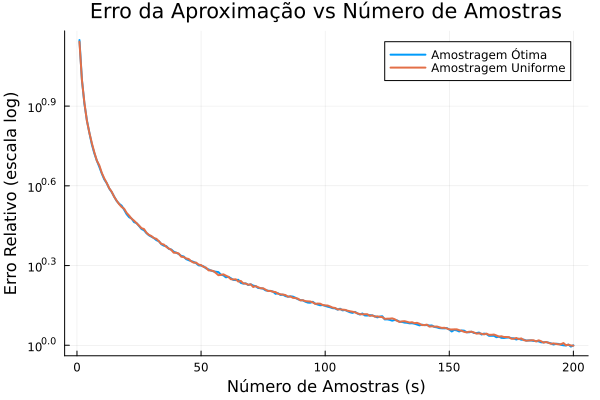
\includegraphics[width=0.8\textwidth]{result-randn.png}
  \caption{Erro relativo da aproximação do produto $AB$ via amostragem probabilística.}
\end{figure}

Em seguida, realizamos os testes gerando as matrizes $A$ e $B$ a partir de matrizes com distribuição uniforme e escalando os resultados obtidos por pesos entre $0.1$ e $100$, ocasionando em matrizes com colunas com normas com maior variação, resultando assim em um experimento que apresenta o resultado esperado. O teste foi realizado com a geração de $100$ matrizes $A$ e $B$ aleatórias e diferentes, tirando no final a média dos resultados obtidos.

\begin{figure}[H]
  \centering
  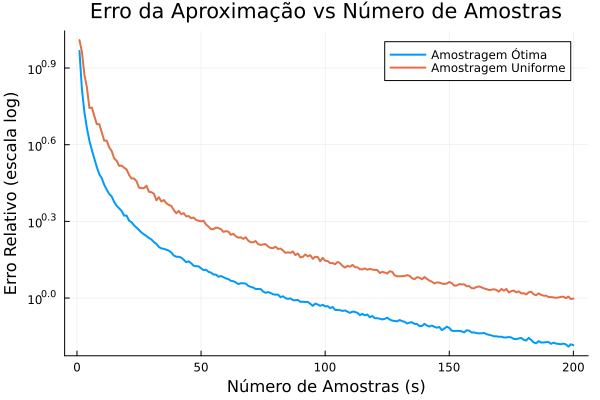
\includegraphics[width=0.8\textwidth]{result-rand_scaled.png}
  \caption{Erro relativo da aproximação do produto $AB$ via amostragem probabilística.}
\end{figure}

Ambas as imagens representam no eixo $y$ o erro relativo de aproximação obtido (em escala logarítmica), calculado pela fórmula \[\dfrac{\fnorm{AB - \bar{AB}}}{\fnorm{AB}},\] e no eixo $x$ o número de mostras. Outro ponto importante de se notar é que o erro apresenta a tendência de diminuir conforme o número de amostras aumenta (visto que uma variância menor fará com que a a amostragem de valores próximos a média real seja mais provável).

Por fim, realizamos um experimento semelhante mas, dessa vez, computando a variância das amostragens ao invés do erro relativo. O teste também foi realizado a partir de $100$ matrizes $A$ e $B$ aleatórias e diferentes, tirando a média dos resultados obtidos no final.

\begin{figure}[H]
  \centering
  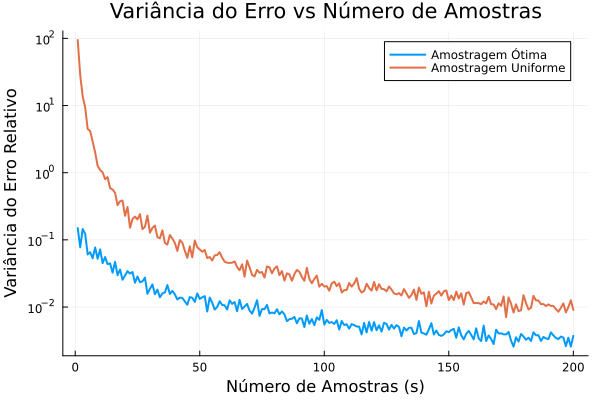
\includegraphics[width=0.8\textwidth]{result-variance.png}
  \caption{Variância amostragem probabilística.}
  \label{fig:second-experiment}
\end{figure}


  %->8-------------------------------------------------8<-%
  \newpage
  \nocite{*}
  \printbibliography
  \addcontentsline{toc}{chapter}{Bibliografia}
  %->8-------------------------------------------------8<-%

\end{document}